\documentclass{article}
\usepackage[utf8]{inputenc}
\usepackage{amstext}
\usepackage{amsmath}
\usepackage{amsfonts}
\usepackage{graphicx}
\usepackage[margin=1in, paperwidth=8.5in, paperheight=11in]{geometry}
\usepackage{gensymb}
\usepackage{indentfirst}
\usepackage{textcomp}
\usepackage{upgreek }
\usepackage{siunitx}
\usepackage{enumitem}

\usepackage[american]{circuitikz}

\title{Circuits Postlab 5}
\author{Byron Wasti}
\date{March 2017}

\begin{document}
\maketitle

\begin{figure}[h]
    \centering
    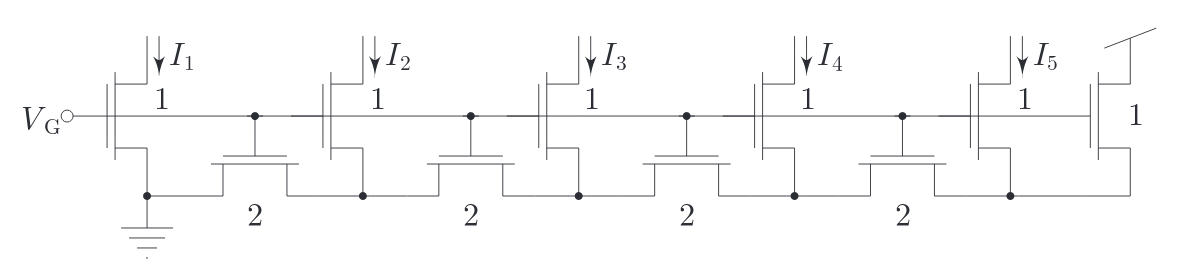
\includegraphics[width=\textwidth]{../circuits}
    \caption{Ladder network of nMOS transistors}
    \label{fig:one}
\end{figure}

\section{Problem 1}

Looking at the rightmost transistor in the ladder shown in Figure \ref{fig:one}: since the strength ratio is $1$, and it has the same $V_{GS}$ as the transistor passing $I_5$, then this transistor must have a current of $I_5$. Thus, the two transistors act as a single $n$MOS transistor with a strength ratio of $2$. This equivalent transistor is then in series with a transistor of strength ratio $2$, thus making two matched transistors of strength ratio $2$ in series. Thus, the equivalent transistor for all three of the rightmost transistors is simply a transistor of strength ratio $1$ passing a current of $2I_5$ (due to KCL).

If we continue this equivalent-transistor analysis, we find that the transistor passing $I_4$ must be passing the same current as the equivalent transistor for the rightmost three transistors. We then have $I_4 = 2I_5$. This pattern continues, and we can find an equation relating the transistor currents:

\begin{equation}
    I_i = 2I_{i+1}
\end{equation}

This equation holds for all currents, except for the second to the rightmost transistor (in this example, the one passing $I_5$) since there is no $i+1$ for this transistor.\\

This relationship does not depend on whether the currents are in weak, moderate or strong inversion, since as we found in the prelab, matched $n$MOS transistors in series and parallel do not depend on the inversion level. This ladder can be extended to have more outputs while maintaining the general relationship we found by simply adding a transistor of strength-ratio $2$ in series (right before the rightmost transistor with Drain at $V_{dd}$) and a transistor of strength-ratio $1$ in series with our added transistor of strength-ratio $2$, and supplying this new transistor with a current $I_{n+1}$.



\end{document}

